\section{From a regular expression to a finite state automaton}

There are a few algorithms to transform a regular expression into an automaton, which differ as for automaton characteristic. 
The three main methods are:
\begin{enumerate}
    \item Thompson (or structural method): it decomposes the regular expression into subexpressions, until it reaches the terminal symbols, and then it constructs the subexpression recognizers, connects them and builds up a network of recognizers that implement the union, concatenation and star operators.
    \item Glushkov-McNaughton-Yamada: it constructs a nondeterministic recognizer without spontaneous moves, but with multiple transitions.
    \item Berry-Sethi method: it constructs a deterministic recognizer without spontaneous moves, but of size often larger than Thompson. 
\end{enumerate}

\subsection*{Thompson structural method}
The Thompson structural method modifies the original automaton to have unique initial and final states.
It is is based on the correspondence of regular expression and recognizer automaton. 
The rules used to find the automaton are the following: 
\begin{table}[H]
    \centering
    \begin{tabular}{cc}
    \hline
    Recognizers of atomic regular expressions & \begin{minipage}{.4\textwidth}\centering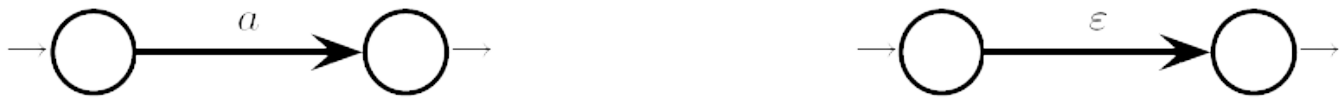
\includegraphics[width=\linewidth, height=6mm]{images/t1.png}\end{minipage} \\ \hline
    Concatenation of two regular expressions  & \begin{minipage}{.4\textwidth}\centering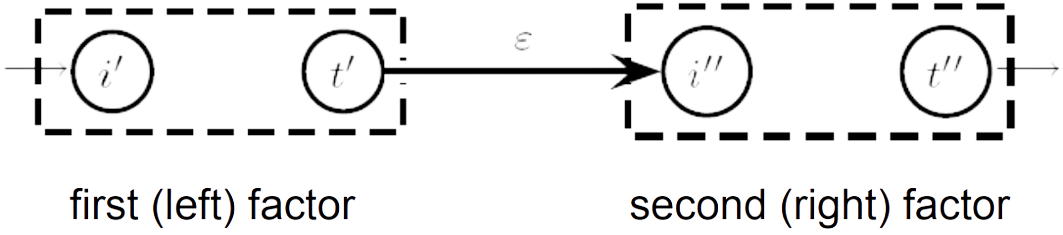
\includegraphics[width=\linewidth, height=15mm]{images/t2.png}\end{minipage} \\ \hline
    Union of two regular expressions          & \begin{minipage}{.4\textwidth}\centering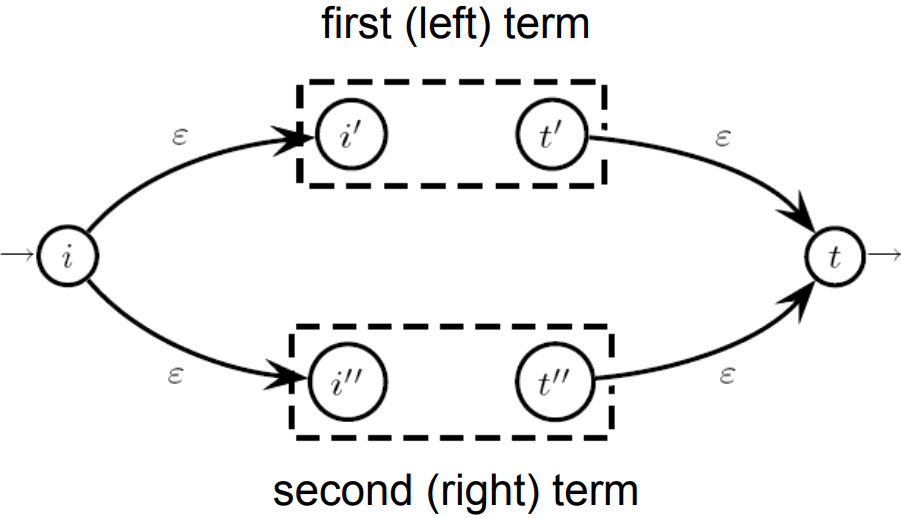
\includegraphics[width=\linewidth, height=37mm]{images/t3.png}\end{minipage} \\ \hline
    Star closure of a regular expression      & \begin{minipage}{.4\textwidth}\centering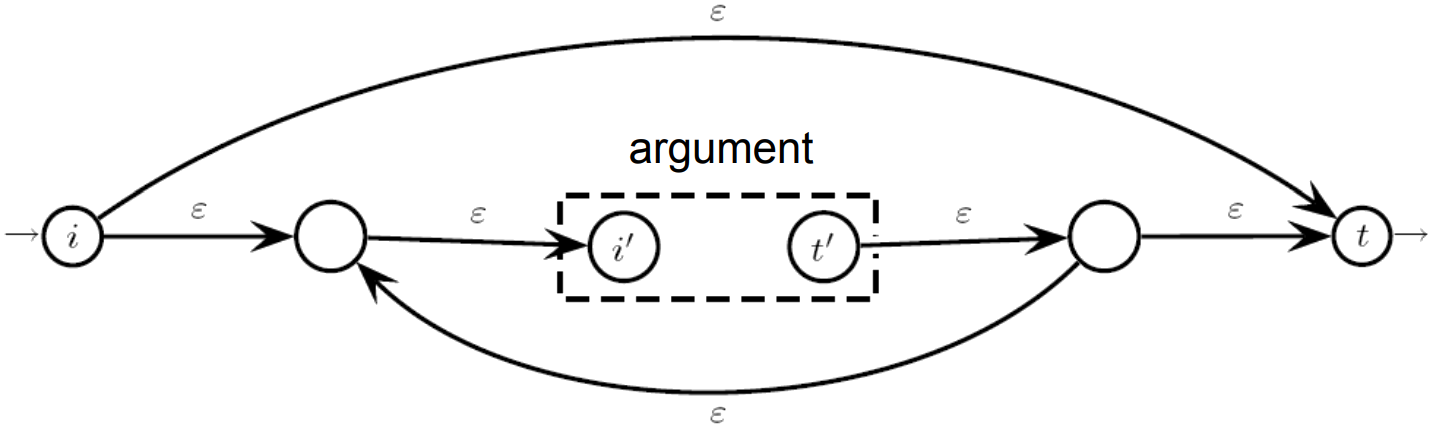
\includegraphics[width=\linewidth, height=25mm]{images/t4.png}\end{minipage} \\ \hline
    \end{tabular}
\end{table}
In general the outcome of the Thompson method is a non-deterministic automaton with spontaneous moves. 
The method is an application of the closure properties of the regular languages under the operations of union, concatenation and star.
\begin{example}
    Consider the regular expression $(a \cup \varepsilon)b^{*}$. 
    It is possible to rewrite the same regular expression with symbols and subexpressions indexing, that is: 
    \[\left(_1\left(_2\left(_3a\right)_4 \cup \left(_5\varepsilon\right)_6\right)_7\left(_8\left(_9b\right)_{10}\right)_{11}^{*}\right)_{12}\]
    The corresponding structure tree is as follows: 
    \begin{figure}[H]
        \centering
        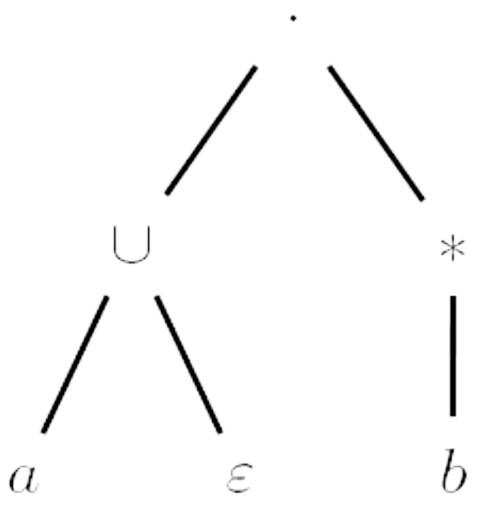
\includegraphics[width=0.15\linewidth]{images/st.png}
    \end{figure}
    By applying the rules of the previous table we obtain the following automaton: 
    \begin{figure}[H]
        \centering
        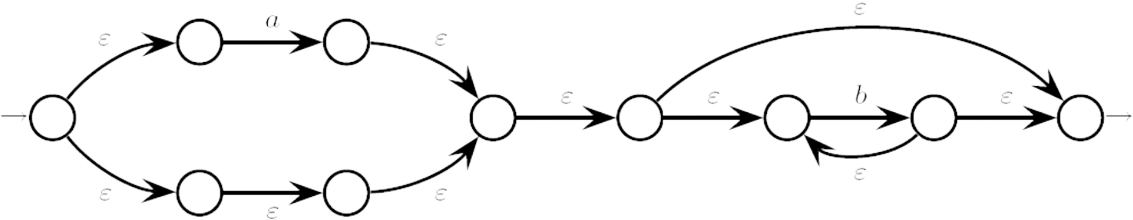
\includegraphics[width=0.75\linewidth]{images/at.png}
    \end{figure}
    The automaton found can be optimized to avoid redundant states. 
\end{example}

\subsection*{Glushkov-McNaughton-Yamada algorithm}
The GMY algorithm constructs the automaton equivalent to a given regular expression, with states that are in a one-to-one correspondence with the generators that occur in the regular expression. 

Given a language $L$ over the alphabet $\Sigma$ we can define: 
\begin{itemize}
    \item The set of initials: $\textnormal{Ini}(L)=\{a \in \Sigma | a\Sigma^{*}\cap L \neq \varnothing\}$. 
    \item The set of finals: $\textnormal{Fin}(L)=\{a \in \Sigma | \Sigma^{*}a\cap L \neq \varnothing\}$.
    \item The set of digrams: $\textnormal{Dig}(L)=\{x \in \Sigma^{2} | \Sigma^{*}x\Sigma^{*} \cap L \neq \varnothing\}$.
    \item The set of forbidden digrams: $\overline{\textnormal{Dig}(L)}=\Sigma^{2} \backslash\textnormal{Dig}(L)$
\end{itemize}
To compute the sets of initials, finals, and digrams we use the following rules: 
\begin{table}[H]
    \centering
    \begin{tabular}{l}
    \hline
    \textbf{Set of initials}                                                                                                                 \\ \hline
    $\textnormal{Ini}(\varnothing)=\varnothing$                                                                                              \\
    $\textnormal{Ini}(\varepsilon)=\varnothing$                                                                                              \\
    $\textnormal{Ini}(a)=\{a\} \textnormal{ for every character }a$                                                                          \\
    $\textnormal{Ini}(e \cup e^{'})=\textnormal{Ini}(e) \cup \textnormal{Ini}(e^{'})$                                                        \\
    $\textnormal{Ini}(e \cdot e^{'})=\textnormal{if Null}(e) \textnormal{ then Ini}(e)\cup\textnormal{Ini}(e^{'}) \textnormal{ else Ini}(e)$ \\
    $\textnormal{Ini}(e^{*})=\textnormal{Ini}(e^{+})=\textnormal{Ini}(e)$                                                                    \\ \hline
    \end{tabular}
\end{table}
\begin{table}[H]
    \centering
    \begin{tabular}{l}
    \hline
    \textbf{Set of finals}                                                                                                                              \\ \hline
    $\textnormal{Fin}(\varnothing)=\varnothing$                                                                                                         \\
    $\textnormal{Fin}(\varepsilon)=\varnothing$                                                                                                         \\
    $\textnormal{Fin}(a)=\{a\} \textnormal{ for every character }a$                                                                                     \\
    $\textnormal{Fin}(e \cup e^{'})=\textnormal{Fin}(e) \cup \textnormal{Fin}(e^{'})$                                                                   \\
    $\textnormal{Fin}(e \cdot e^{'})=\textnormal{if Null}(e^{'}) \textnormal{ then Fin}(e)\cup\textnormal{Fin}(e^{'}) \textnormal{ else Fin}(e^{'})$    \\
    $\textnormal{Fin}(e^{*})=\textnormal{Fin}(e^{+})=\textnormal{Fin}(e)$                                                                               \\ \hline
    \end{tabular}
\end{table}
\begin{table}[H]
    \centering
    \begin{tabular}{l}
    \hline
    \textbf{Set of digrams}                                                                                                                              \\ \hline
    $\textnormal{Dig}(\varnothing)=\varnothing$                                                                                                         \\
    $\textnormal{Dig}(\varepsilon)=\varnothing$                                                                                                         \\
    $\textnormal{Dig}(a)=\varnothing \textnormal{ for every character }a$                                                                                     \\
    $\textnormal{Dig}(e \cup e^{'})=\textnormal{Dig}(e) \cup \textnormal{Dig}(e^{'})$                                                                   \\
    $\textnormal{Dig}(e \cdot e^{'})=\textnormal{Dig}(e) \cup \textnormal{Dig}(e^{'}) \cup \textnormal{Fin}(e) \cdot \textnormal{Ini}(e^{'})$    \\
    $\textnormal{Dig}(e^{*})=\textnormal{Dig}(e^{+})=\textnormal{Dig}(e) \cup \textnormal{Fin}(e) \cdot \textnormal{Ini}(e)$                                                                               \\ \hline
    \end{tabular}
\end{table}
\begin{definition}
    The language $L$ is called \emph{locally testable}, if and only if it satisfies the following identity: 
    \[L\backslash\{\varepsilon\}=\{x|\textnormal{Ini}(x)\in \textnormal{Ini}(L) \land \textnormal{Fin}(x)\in \textnormal{Fin}(L)\land \textnormal{Dig}(x)\subseteq \textnormal{Dig}(L)\}\]
\end{definition}
\begin{example}
    Consider the language $L_1=(abc)^{*}$. 
    The set defined above in this case are: 
    \begin{itemize}
        \item $\textnormal{Ini}(L_1)=\{a\}$.
        \item $\textnormal{Fin}(L_1)=\{c\}$.
        \item $\textnormal{Dig}(L_1)=\{ab,bc,ca\}$.
        \item $\overline{\textnormal{Dig}(L)}=\{aa,ac,ba,bb,cb,cc\}$
    \end{itemize}
\end{example}
To design the recognizer of a local language we scan the input string from left to right and check whether: the initial character belongs to the set Ini, every digram belongs to the set Dig, and the final character belongs to the set Fin. 
The string is accepted if, and only if, all the above checks succeed. 

We can implement the above recognizer by resorting to a sliding window with a width of two characters, which is shifted over the input string from left to right.
At each shift step the window contents are checked, and if the window reaches the end of the string and all the checks succeed, then the string is accepted, otherwise it is rejected. 
This sliding window algorithm is simple to implement by means of a nondeterministic automaton. 

Given the sets Ini, Fin and Dig, the corresponding recognizer has:
\begin{itemize}
    \item Initial states: $q_0 \cup \Sigma$.
    \item Final states: Fin.
    \item Transitions: $q_0 \overset{a}{\rightarrow}a$ if $a \in$ Ini, and $b \overset{a}{\rightarrow}b$ if $ab \in$ Dig.
\end{itemize}
If the language contains the empty string, the initial state $q_0$ is final as well.
\begin{example}
    The recognizer automaton for the language $L_1=(abc)^{*}$ is as follows: 
    \begin{figure}[H]
        \centering
        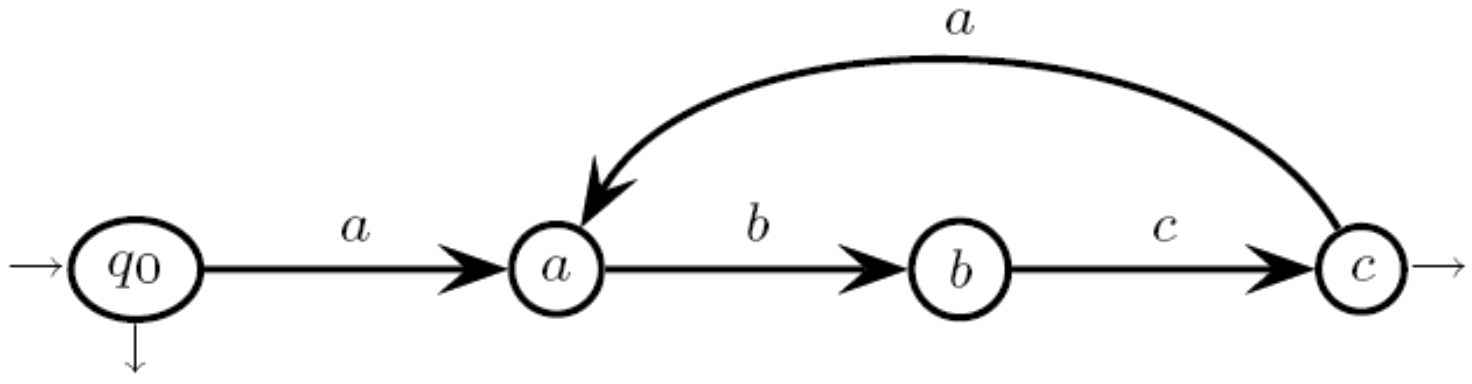
\includegraphics[width=0.5\linewidth]{images/local.png}
    \end{figure}
\end{example}
\begin{definition}
    A regular expression is said to be \emph{linear} if there is not any repeated generator. 
\end{definition}
\begin{property}
    The languages generated by linear regular expressions are local. 
\end{property}
Linearity implies the regular expression subexpressions are defined over disjoint alphabets.
But a regular expression is the composition of its subexpressions, thus the language of a linear regular expression is local as a consequence of the closures of the local languages over disjoint alphabets. 
Notice that the opposite implication does not hold
This implies that constructing the recognizer for a generic regular language reduces to the problem of finding the characteristic local sets Ini, Fin, Dig of such a generic language, provided the alphabet is slightly modified. 

To check whether a regular expression $e$ generates the empty string we can use the Null$(e)$ operator, that is true when the empty string is in the regular expression, false otherwise. 
It works as follows: 
\begin{itemize}
    \item $\textnormal{Null}(\varnothing)=\textnormal{false}$. 
    \item $\textnormal{Null}(\varepsilon)=\textnormal{true}$. 
    \item $\textnormal{Null}(a)=\textnormal{false for every character } a$.
    \item $\textnormal{Null}(e \cup e^{'})=\textnormal{Null}(e) \lor \textnormal{Null}(e^{'})$.
    \item $\textnormal{Null}(e \cdot e^{'})=\textnormal{Null}(e) \land \textnormal{Null}(e^{'})$.
    \item $\textnormal{Null}(e^{*})=\textnormal{true}$. 
    \item $\textnormal{Null}(e^{+})=\textnormal{Null}(e)$. 
\end{itemize}
The idea of the GMY algorithm, based on the linear regular expressions is the following: 
\begin{enumerate}
    \item Enumerate the regular expression e and obtain the linear regular expression $e_{\#}$. 
    \item Compute the three characteristic local sets Ini, Fin and Dig of $e_{\#}$.
    \item Design the recognizer of the local language generated by $e_{\#}$.
    \item Cancel the indexing and thus obtain the recognizer of $e$.
\end{enumerate}
\begin{example}
    Consider the regular expression $e=(ab)^{*}a$.
    To apply the GMY algorithm we follow these steps: 
    \begin{enumerate}
        \item Enumerate the regular expression, obtaining: 
            \[e_{\#}=(a_1b_2)^{*}a_3\]
        \item Compute the sets:
            \begin{itemize}
                \item $\textnormal{Ini}(e)=\{a\}$.
                \item $\textnormal{Fin}(e)=\{a\}$.
                \item $\textnormal{Dig}(e)=\{ab,ba\}$.
            \end{itemize}
        \item Construct the recognizer for the numbered expression: 
            \begin{figure}[H]
                \centering
                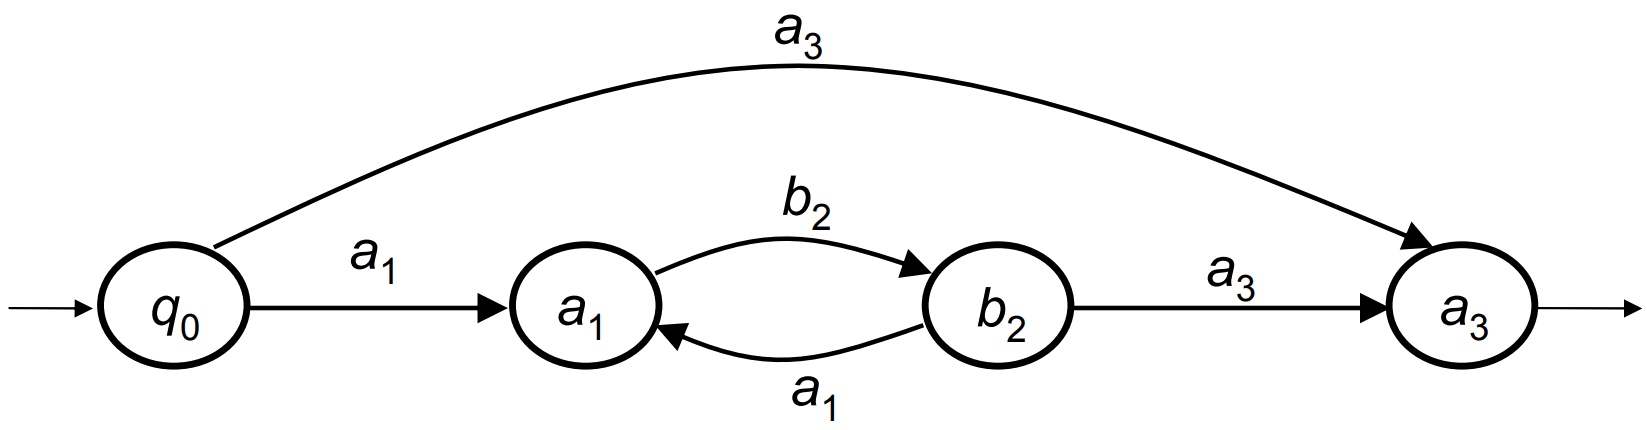
\includegraphics[width=0.5\linewidth]{images/gmy1.png}
            \end{figure}
        \item Remove the enumeration: 
            \begin{figure}[H]
                \centering
                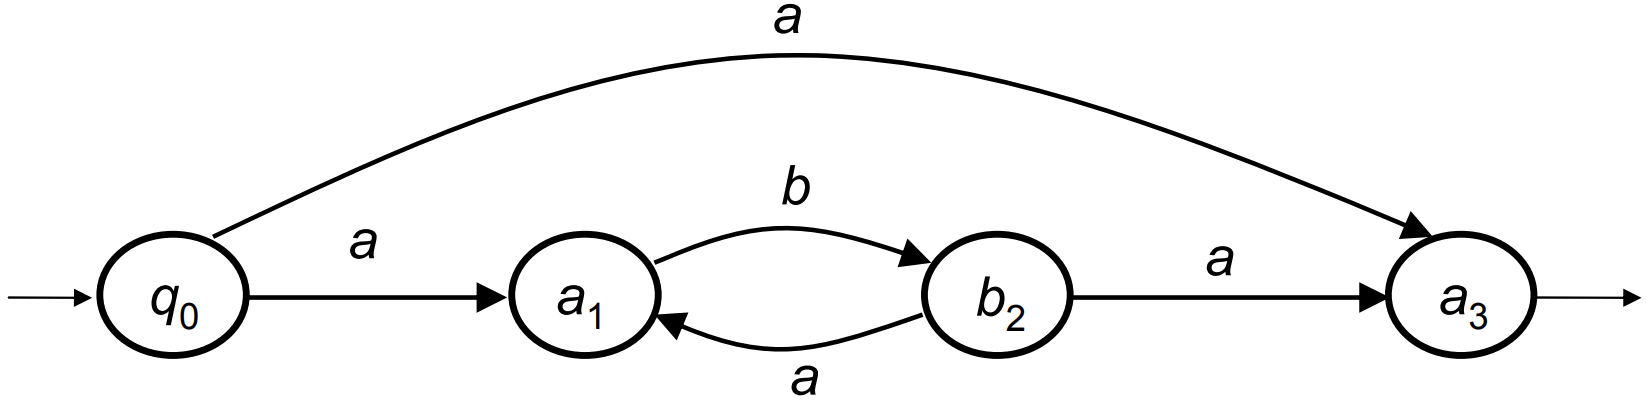
\includegraphics[width=0.5\linewidth]{images/gmy2.png}
            \end{figure}
    \end{enumerate}
    The result is a non-deterministic automaton without spontaneous moves, with as many states as the occurrences of generators in the regexp are, and one more state. 
\end{example}

\subsection*{Berry-Sethi method}
In order to obtain the deterministic recognizer, we can just apply the subset construction to the non-deterministic recognizer built by the GMY algorithm. 
However, there is a more direct algorithm called Berry-Sethi.
The idea at the base of this algorithm is the following: 
\begin{enumerate}
    \item Consider the end-marked regular expression $e \dashv$ instead of the original regular expression $e$.
    \item Let $e$ be a regular expression over the alphabet $\Sigma$, and let $e_{\#}$ be the numbered version of $e$ over $\Sigma_{\#}$ with predicate Null and local sets Ini, Fin and Dig. 
    \item Define the set Fol as follows: 
        \begin{enumerate}
            \item $\textnormal{Fol}(c_{\#}) \in \mathcal{P} (\Sigma_{\#} \cup \{\dashv\})$. 
            \item $\textnormal{Fol}(\dashv)=\varphi$.
            \item $\textnormal{Fol}(a_i)=\{b_j|a_ib_j \in \textnormal{Dig}(e_{\#}\dashv)\}$ where $a_i$ and $b_j$ may coincide. 
        \end{enumerate} 
    \item Apply the following algorithm. 
\end{enumerate}
\begin{algorithm}[H]
    \caption{Berry-Sethi algorithm}
        \begin{algorithmic}[1]
            \State $q_0 \leftarrow Ini(e_{\#} \dashv)$
            \State $Q \leftarrow \{q_0\}$
            \State $\delta \leftarrow \varnothing$
            \While {$\exists q \in Q$ such that $q$ is unmarked}
                \State mark state $q$ as visited
                \For {each character $c \in \Sigma$}
                    \State $q^{'} \leftarrow \bigcup_{\forall c_{\#} \in \Sigma_{c_{\#}}}Fol(c_{\#})$
                    \If {$q^{'} \neq \varnothing$}
                        \If {$q^{'} \notin Q$}
                            \State set $q^{'}$ as a new unmarked state
                            \State $Q \leftarrow Q \cup \{q^{'}\}$
                        \EndIf
                        \State $\delta \leftarrow Q \cup \{q^{'}\}$
                    \EndIf
                \EndFor
            \EndWhile
        \end{algorithmic}
\end{algorithm}
\begin{example}
    Given the language $L=(a|bb)^{*}(ac)^{+}$ apply the BS algorithm. First we enumerate the string: 
    \[e_{\#}=(a_1|b_2b_3)^{*}(a_4c_5)^{+} \dashv\]
    The characteristic sets are: 
    \begin{itemize}
        \item $\textnormal{Ini}(e_{\#})=\{a_1,b_2,a_4\}$.
        \item $\textnormal{Fin}(e_{\#})=\{\dashv\}$.
        \item $\textnormal{Dig}(e_{\#})=\{a_1a_1,a_1b_2,a_1a_4,b_2b_3,b_3a_1,b_3b_2,b_3a_4,a_4c_5,c_5a_4,c_5\dashv\}$.
    \end{itemize}
    The table of the followers is as follows: 
    \begin{table}[H]
        \centering
        \begin{tabular}{cc}
        \hline
        \textbf{$\boldsymbol{c_{\#}}$} & \textbf{Fol$(\boldsymbol{c_{\#}})$} \\ \hline
        $a_1$                          & $a_1b_2a_4$                         \\
        $b_2$                          & $b_3$                               \\
        $b_3$                          & $a_1b_2a_4$                         \\
        $a_4$                          & $c_5$                               \\
        $c_5$                          & $a_4\dashv$                         \\ \hline
        \end{tabular}
    \end{table}
    The resulting automaton is as follows: 
    \begin{figure}[H]
        \centering
        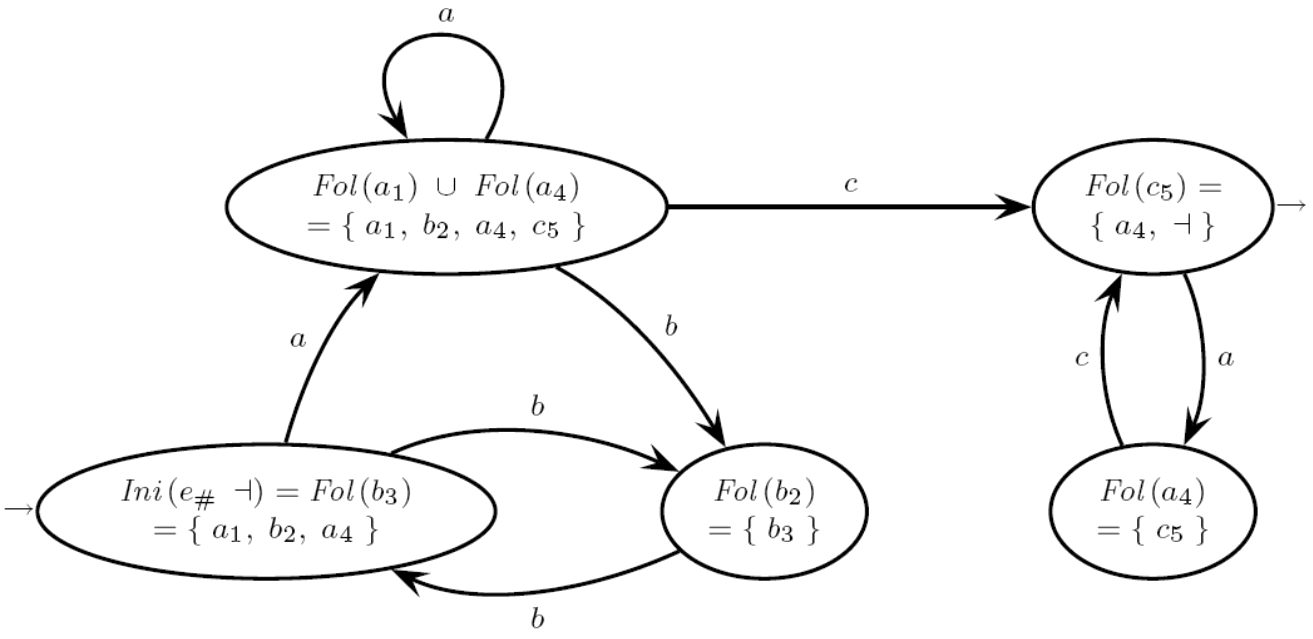
\includegraphics[width=0.7\linewidth]{images/bs.png}
    \end{figure}
\end{example}

The Berry-Sethi algorithm can be also used to transform a nondeterministic automaton into a deterministic one. 
The steps are: 
\begin{enumerate}
    \item Enumerate the elements on the arcs. 
    \item Create the followers table. 
    \item Recreate the automaton by using the followers table. 
\end{enumerate}
\begin{example}
    Consider the following automaton: 
    \begin{figure}[H]
        \centering
        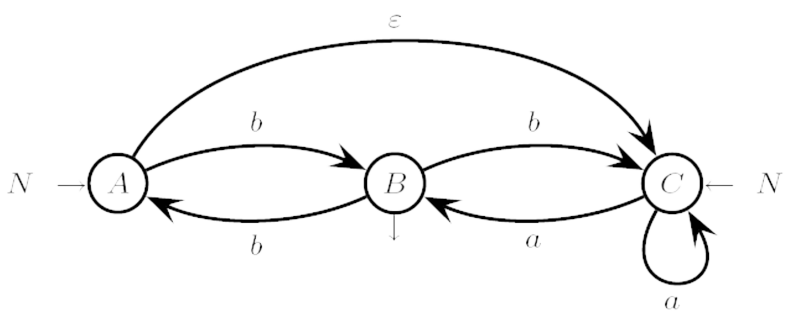
\includegraphics[width=0.5\linewidth]{images/bs1.png}
    \end{figure}
    Its numbered version is the following: 
    \begin{figure}[H]
        \centering
        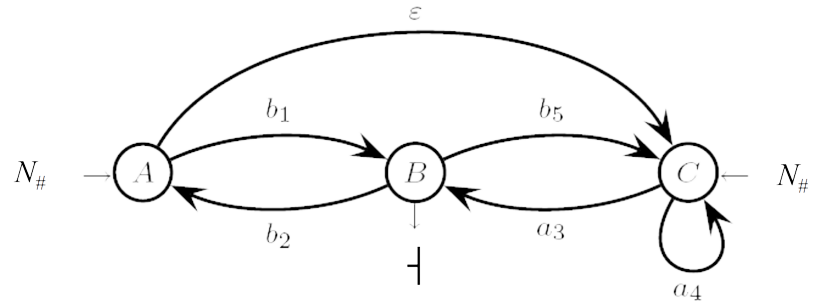
\includegraphics[width=0.5\linewidth]{images/bs2.png}
    \end{figure}
    The follower table is: 
    \begin{table}[H]
        \centering
        \begin{tabular}{cc}
        \hline
        \textbf{$\boldsymbol{c_{\#}}$} & \textbf{Fol$(\boldsymbol{c_{\#}})$} \\ \hline
        $b_1$                          & $b_2b_5\dashv$                      \\
        $b_2$                          & $b_1a_3a_4$                         \\
        $a_3$                          & $b_2b_5\dashv$                      \\
        $a_4$                          & $a_3a_4$                            \\
        $b_5$                          & $a_3a_4$                            \\ \hline
        \end{tabular}
    \end{table}
    The final deterministic automaton is: 
    \begin{figure}[H]
        \centering
        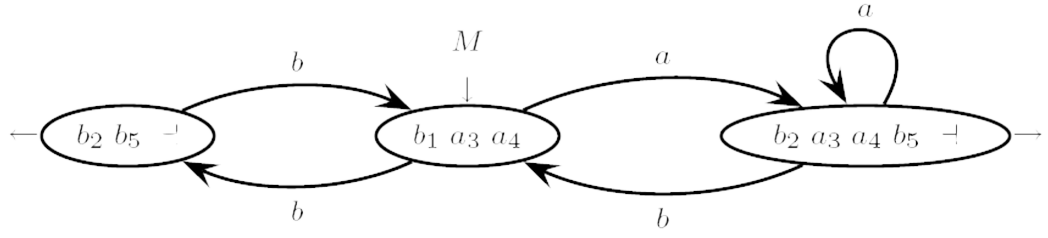
\includegraphics[width=0.7\linewidth]{images/bs3.png}
    \end{figure}
\end{example}